\section{A solution: Pulp}
\label{sec:pulp}

Pulp is a tool ``for managing software repositories and their
associated content, such as packages, errata, and
distributions''~\cite{Dob11}.  It is, as noted, the spiritual
successor to Spacewalk, and so implements the vast majority of
Spacewalk's repository management features without the dependency on
Oracle.

Pulp's usage model involves syncing multiple upstream repositories
locally; these repositories can then be \emph{cloned}, which uses hard
links to sync them locally with almost no disk space used.  This
allows us to sync a repository once, then duplicate it as many times
as necessary to support multiple teams and multiple stability levels.
The sync process supports \emph{filters}, which allow us to blacklist
or whitelist packages and thus exclude ``impactful'' packages from
automatic updates.

Pulp also supports manually adding packages to and removing packages
from repositories, so we can later update a given package across all
machines that use a repository with a single command.  Adding and
removing also tracks dependencies, so it's not possible to add a
package to a repository without adding the dependencies necessary to
install it.\endnote{This is actually only true if the package is being
  added from another repository; it is possible to add a package
  directly from the filesystem, in which case dependency checking
  is not performed.  This is not a use case for us, though.}

\subsection{Workflow}

Pulp provides us with the framework to implement a solution to the
problem outlined earlier, but even as featureful as it is it remains a
fairly basic tool.  Our workflow -- enforced by the features Pulp
provides, by segregating repositories, by policy, and by a nascent
in-house web interface -- provides the bulk of the solution.  Briefly,
we segregate repositories by tier to test packages before site-wide
roll-outs, and by team to ensure operational separation.  Packages are
automatically synced between tiers based on package filters, which
blacklist certain packages that must be promoted manually.  This
ensures that most packages benefit from up to two weeks of community
testing before being deployed site-wide, and packages that we have
judged to be more potentially ``impactful'' from more focused local
testing as well.

\subsubsection{Tiered Repositories}

We maintain different repository sets for different ``levels'' of
stability.  We chose to maintain three tiers:

\begin{description}
\item[\texttt{live}] Synced daily from upstream repositories; not used
  on any machines, but maintained due to operational requirements
  within Pulp\endnote{In Pulp, filters can only be applied to
    repositories with local feeds.} and for reference.
\item[\texttt{unstable}] Synced daily from \texttt{live}, with the
  exception of selected ``impactful'' packages (more about which
  shortly), which can be manually promoted from \texttt{live}.
\item[\texttt{stable}] Synced daily from \texttt{unstable}, with the
  exception of the same ``impactful'' packages, which can be manually
  promoted from \texttt{unstable}.
\end{description}

This three-tiered approach guarantees that packages in \texttt{stable}
are at least two days old, and ``impactful'' packages have been in
testing by machines using the \texttt{unstable} branch.  When a
package is released from upstream and sync to public mirrors, those
packages are pulled down into local repositories. From then on the
package is under the control of Pulp. Initially, a package is
considered unstable and is only deployed to those systems that look at
the repositories in the \texttt{unstable} tier. After a period of
time, the package is then promoted into the \texttt{stable}
repositories, and thus to production machines.

In order to ensure that packages in \texttt{unstable} receive ample
testing before being promoted to \texttt{stable}, we divide machines
amongst those two tiers thusly:

\begin{itemize}
\item All internal test machines -- that is, all machines whose sole
  purpose is to provide test and development platforms to customers
  within the group -- use the \texttt{unstable} branch.  Many of these
  machines are similar, if not identical, to production or external
  test machines.
\item Where multiple identical machines exist for a single purpose,
  whether in an active-active or active-passive configuration, exactly
  one machine will use the \texttt{unstable} branch and the rest will
  use the \texttt{stable} branch.
\end{itemize}

Additionally, we maintain separate sets of repositories, branched
from \texttt{live}, for different teams or projects that require
different patching policies appropriate to the needs of those teams or
projects.  Pulp has strong built-in ACLs that support these divisions.

In order to organize multiple tiers across multiple groups, we use a
strict convention to specify the repository ID, which acts as the
primary key across all repositories\endnote{This may change in future
  versions of Pulp, as multiple users, ourselves included, have asked
  for stronger grouping functionality~\cite{Dob11-2}.}, namely:

{\tt \small
\begin{verbatim}
<team name>-<tier>-<os name>-<os version>-
    <arch>-<repo name>
\end{verbatim}
}

For example,\\
\texttt{infra-unstable-centos-6-x86\_64-updates} would
denote the Infrastructure team's \texttt{unstable} tier of the 64-bit
CentOS 6 ``updates'' repository.  This allows us to tell at a glance
the parent-child relationships between repositories.

\subsubsection{Sync Filters}

The syncs between the \texttt{live} and \texttt{unstable} and between
\texttt{unstable} and \texttt{stable} tiers are mediated by
filters\endnote{As noted earlier, in Pulp, filters can only be applied
  to repositories with local feeds, so no filter mediates the sync
  between upstream and \texttt{live}.}.  Filters are regular
expression lists of packages to either blacklist from the sync, or
whitelist in the sync; in our workflow, only blacklists are used.  A
package filtered from the sync may still remain in the repository;
that is, if we specify \texttt{\^{}kernel(-.*)?} as a blacklist filter,
that does not remove \texttt{kernel} packages from the repository, but
rather refuses to sync new \texttt{kernel} packages from the
repository's parent.  This is critical to our version-pegging system.

Given our needs, whitelist filters are unnecessary; our systems tend
to fall into one of two types:

\begin{itemize}
\item Systems where we generally want updates to be installed insofar
  as is reasonable, with some prudence about installing updates to
  ``impactful'' packages.
\item Systems where, due to vendor requirements, we must set all
  packages to a specific version.  Most often this is in the form of a
  requirement for a minor release of RHEL\endnote{It is lost on many
    vendors that it is unreasonable and foolish to require a specific
    RHEL minor release.  As much work as has gone into this solution,
    it is still less than would be required to convince most vendors
    of this fact, though.}, in which case there are no updates we wish
  to install on an automatic basis.  (We may wish to update specific
  packages to respond to security threats, but that happens with
  manual package promotion, not with a sync; this workflow gives us
  the flexibility necessary to do so.)
\end{itemize}

A package that may potentially cause issues when updated can be
blacklisted on a per-team basis\endnote{Technically, filters can be
  applied on a per-repository basis, so black- and whitelists can be
  applied to individual repositories.  This is very rare in our
  workflow, though.}. Since the repositories are hierarchically
tiered, a package that is blacklisted from the \texttt{unstable} tier
will never make it to the \texttt{stable} tier.

\subsubsection{Manual Package Promotion and Removal}

The lynchpin of this process is manually reviewing packages that have
been blacklisted from the syncs and \emph{promoting} them manually as
necessary.  For instance, if a filter for a set of repositories
blacklisted \texttt{\^{}kernel(-.*)?} from the sync, without manually
promoting new kernel packages no new kernel would ever be installed.

To accomplish this, we use Pulp's \emph{add package} functionality,
exposed via the REST API as a POST
to\\ \texttt{/repositories/<id>/add\_package/}, via the Python client
API as\\ \texttt{pulp.client.api.repository.RepositoryAPI.
  add\_package()}, and via the CLI as \texttt{pulp-admin repo
  add\_package}.  In the CLI implementation, \texttt{add\_package}
follows dependencies, so promoting a package will promote everything
that package requires that is not already in the target repository.
This helps ensure that each repository stays consistent even as we
manipulate it to contain only a subset of upstream packages\endnote{It
  is true that our approach does not \emph{guarantee} consistency.  A
  repository sync might result in an inconsistency if a package that
  was not listed on that sync's blacklist required a package that was
  listed on the blacklist.  In practice this can be limited by using
  regular expressions to filter families of packages (e.g.,
  \texttt{\^{}mysql.*} or \texttt{\^{}(.*-)?mysql.*} to blacklist all
  MySQL-related packages rather than just blacklisting the
  \texttt{mysql-server} package itself}.

Conversely, if a package is deployed and is later found to cause
problems it can be removed from the tier and the previous version, if
such is available in the repository, will be (re)installed.  Bcfg2
will helpfully flag machines where a newer package is installed than
is available in that machine's repositories, and will try to downgrade
packages appropriately.  Pulp can be configured to retain old packages
when it performs a sync; this is helpful for repositories like EPEL
that remove old packages themselves, and guarantees that a
configurable number of older package versions are available to fall
back on.

The \emph{remove package} functionality is exposed via Pulp's REST API
as a POST to\\ \texttt{/repositories/<id>/delete\_package/}, via the
Python client API
as\\ \texttt{pulp.client.api.repository.RepositoryAPI.
  remove\_package()}, and via the CLI as \texttt{pulp-admin repo
  remove\_package}.  As with \texttt{add\_package}, the CLI
implementation follows dependencies and will try to remove packages
that require the package being removed; this also helps ensure
repository consistency.

Optimally, security patches are applied 10 or 30 days after the
initial patch release~\cite{BACWWS02}; this workflow allows us to
follow these recommendations to some degree, promoting new packages to
the \texttt{unstable} tier on an approximately weekly basis.  Packages
that have been in the \texttt{unstable} tier for at least a week are
also promoted to the \texttt{stable} tier every week; in this we
deviate from Beattie et al.'s recommendations somewhat, but we do so
because the updates being promoted to \texttt{stable} have been vetted
and tested by the machines using the \texttt{unstable} tier.

This workflow also gives us something very important: the ability to
install updates across all machines much sooner than the optimal 10-
or 30-day period.  High profile vulnerabilities require immediate
action -- even to the point of imperiling uptime -- and by promoting a
new package immediately to both \texttt{stable} and \texttt{unstable}
tiers we can ensure that it is installed across all machines in our
environment in a timely fashion.

\subsubsection{Selecting ``impactful'' packages}

Throughout this paper, we have referred to ``impactful'' packages --
those to which automatic updates we determined to be particularly
dangerous -- as a driving factor.  Were it not for our reticence to
automatically update all packages, we could have simply used an
automatic update facility -- \texttt{yum-cron} or
\texttt{yum-updatesd} are both popular -- and been done with it.

We didn't feel that was appropriate, though.  For instance, installing
a new kernel can be problematic -- particularly in an environment with
a wide variety of third-party kernel modules and other kernel-space
modifications -- and we wanted much closer control over that process.
We flagged packages as ``impactful'' according to a simple set of
criteria:

\begin{itemize}

\item The kernel, and packages otherwise directly tied to kernel space
  (e.g., kernel modules and Dynamic Kernel Module Support (DKMS)
  packages);

\item Packages that provide significant, customer-facing services.  On
  the Infrastructure team, this included packages like \texttt{bind},
  \texttt{httpd} (and related modules), \texttt{mysql}, and so on.

\item Packages related to InfiniBand and Lustre~\cite{Ora10}; as one
  of the world's largest unclassified Lustre installations, it's very
  important that the Lustre versions on our systems stay in lockstep
  with all other systems in the center.  Parts of Lustre reside
  directly in kernel space, an additional consideration.

\end{itemize}

The first two criteria provided around 20 packages to be excluded -- a
tiny fraction of the total packages installed across all of our
machines.  The vast majority of supporting packages continue to be
automatically updated, albeit with a slight time delay for the
multiple syncs that must occur.

\subsection{Results}

Our approach produces results in a number of areas that are difficult
to quantify: improved automation reduces the amount of time we spend
installing patches; not installing patches immediately improves patch
quality and reduces the likelihood of flawed patches~\cite{BACWWS02};
and increased compartmentalization makes it easier for our diverse
teams to work to different purposes without stepping on toes.  But it
also provides testable, quantifiable improvements: since replacing a
manual update process with Pulp and Bcfg2's automated update process,
we can see that the number of available updates has decreased and
remained low on the machines using Pulp.

\begin{center}
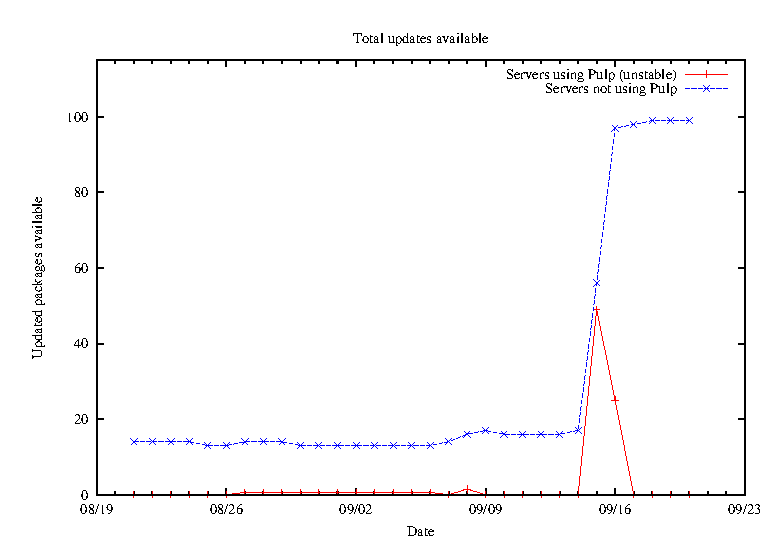
\includegraphics[width=8cm]{updates}
\end{center}

The practice of staging package deployment makes is difficult to
quantify just how out of date a client is, as yum on the client will
only report the number of updates available from the repositories in
\texttt{yum.conf}. To find the number of updates available from
upstream, we collect an aggregate of all the package differences
starting at the client and going up the heirarchy to the upstream
repository.  E.g., for a machine using the \texttt{unstable} tier, we
calculate the number of updates available on the machine itself, and
then the number of updates available to the \texttt{unstable} tier
from the \texttt{live} tier.

The caveat to this approach is when, for instance, a package splits
into two new packages. This results in two new packages, and one
missing package, totaling three ``updates'' according to \texttt{yum
  check-update}, or zero ``updates'' when comparing repositories
themselves, when in reality it is a single package update. For
example, if package \texttt{foo} recieves an update that results in
packages \texttt{foo-client} and \texttt{foo-server}, this could
result in a margin of error of -1 or +2.  This gives a slight
potential benefit to machines using Pulp in our metrics, as updates of
this sort are underestimated when calculating the difference between
repositories, but overestimated when using \texttt{yum} to report on
updates available to a machine.  In practice, this is extremely rare,
though, and should not significantly affect the results.

Ensuring, with a high degree of confidence, that updates are installed
is wonderful, but even more important is ensuring that vulnerabilities
are being mitigated.  Using the data from monthly Nessus~\cite{Ten11}
vulnerability scans, we can see that machines using Pulp do indeed
reap the benefits of being patched with more
frequency:\endnote{Unfortunately long-term data was not available for
  vulnerabilities for a number of reasons: CentOS 5 stopped shipping
  updates in their mainline repositories between July 21st and
  September 14th; the August security scan was partially skipped; and
  Pulp hasn't been in production long enough to get meaningful numbers
  prior to that.  Still, the snapshot of data is compelling.}

\begin{center}
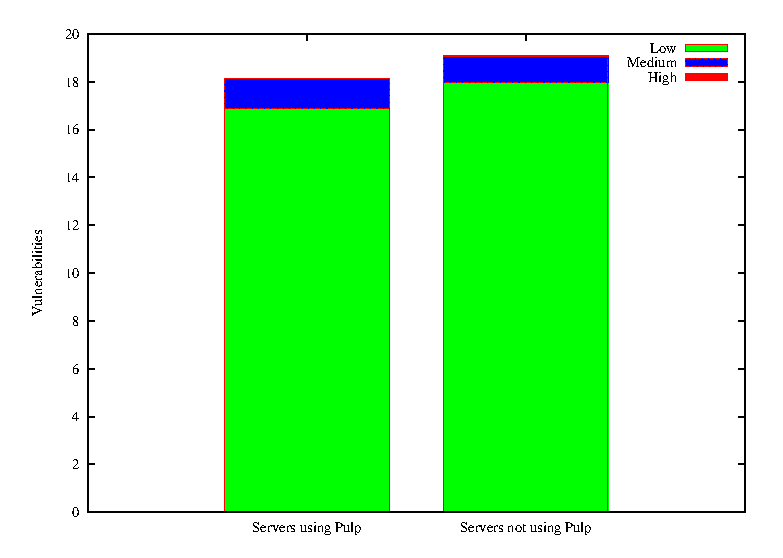
\includegraphics[width=8cm]{vulns}
\end{center}

This graph is artificially skewed against Pulp due to the sorts of
things Nessus scans for; for instance, web servers are more likely to
be using Pulp at this time simply due to our implementation plan, and
they also have disproportionately more vulnerabilities in Nessus
because they have more services exposed.
